%
% leapfrog.tex -- Leap-Frog Ableitung Lösungen
%
% (c) 2018 Prof Dr Andreas Müller, Hochschule Rapperswil
%
\documentclass[tikz]{standalone}
\usepackage{times}
\usepackage{txfonts}
\usepackage[utf8]{inputenc} 
\usepackage{graphics}
\usepackage{ifthen}
\usepackage{color}
\usetikzlibrary{arrows,intersections}
\usetikzlibrary{math}
\begin{document} 
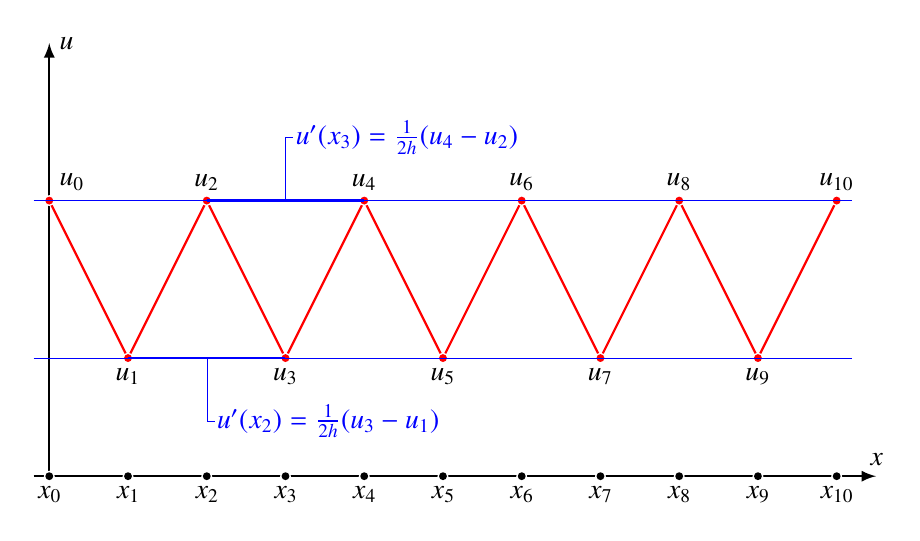
\begin{tikzpicture}[>=latex,thick]

\draw[->] (-0.2,0)--(10.5,0) coordinate[label=$x$];
\draw[->] (0,-0.0)--(0,5.5) coordinate[label={right:$u$}];

\def\oben{3.5}
\def\unten{1.5}

\foreach\x in {0,...,10}{
	\fill[color=white] ({\x},0) circle[radius=0.07];
	\fill ({\x},0) circle[radius=0.05];
	\node at ({\x},0) [below] {$x_{\x}$};
}

\draw[color=red]
(0,\oben)--
(1,\unten)--
(2,\oben)--
(3,\unten)--
(4,\oben)--
(5,\unten)--
(6,\oben)--
(7,\unten)--
(8,\oben)--
(9,\unten)--
(10,\oben);

\fill[color=white] (0,\oben) circle[radius=0.07];
\fill[color=red] (0,\oben) circle[radius=0.05];
\node at (0,\oben) [above right] {$u_0$};
\foreach\x in {2,4,...,10}{
	\fill[color=white] ({\x},\oben) circle[radius=0.07];
	\fill[color=red] ({\x},\oben) circle[radius=0.05];
	\node at ({\x},\oben) [above] {$u_{\x}$};
}

\foreach\x in {1,3,...,9}{
	\fill[color=white] ({\x},\unten) circle[radius=0.07];
	\fill[color=red] ({\x},\unten) circle[radius=0.05];
	\node at ({\x},\unten) [below] {$u_{\x}$};
}

\draw[color=blue,line width=0.1pt] (-0.2,\oben)--(10.2,\oben);
\draw[color=blue] (1,\unten)--(3,\unten);
\draw[color=blue,line width=0.1pt] (2,\unten)--(2,{\unten-0.8})--(2.1,{\unten-0.8});
\node[color=blue] at (2,{\unten - 0.8}) [right] {$u'(x_2) = \frac{1}{2h}(u_3-u_1)$};

\draw[color=blue,line width=0.1pt] (-0.2,\unten)--(10.2,\unten);
\draw[color=blue] (2,\oben)--(4,\oben);
\draw[color=blue,line width=0.1pt] (3,\oben)--(3,{\oben+0.8})--(3.1,{\oben+0.8});
\node[color=blue] at (3,{\oben + 0.8}) [right] {$u'(x_3) = \frac{1}{2h}(u_4-u_2)$};

\end{tikzpicture}
\end{document}
